%!TEX root = forallxsol.tex
%\part{Natural deduction for FOL}
%\label{ch.NDFOL}
%\addtocontents{toc}{\protect\mbox{}\protect\hrulefill\par}

\setcounter{chapter}{31}
\chapter{Basic rules for FOL}\setcounter{ProbPart}{0}
\problempart
The following two `proofs' are \emph{incorrect}. Explain why both are incorrect. Also, provide interpretations which would invalidate the fallacious argument forms the `proofs' enshrine:
\begin{multicols}{2}
	\begin{proof}
		\hypo{Rxx}{\forall x Rxx}
		\have{Raa}{Raa}\Ae{Rxx}
		\have{Ray}{\forall y Ray}\Ai{Raa}
		\have{Rxy}{\forall x \forall y Rxy}\Ai{Ray}
	\end{proof}
\vfill
\noindent\myanswer{When using $\forall$I, you must replace \emph{all} names with the new variable. So line 3 is bogus. As a counterinterpretation, consider the following:
\begin{center}
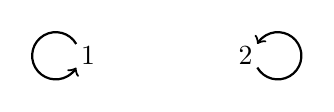
\begin{tikzpicture}
\node (atom4) at (0,0) {1};
\node (atom5) at (2,0) {2};
\draw[->, thick] (atom4)+(-0.15,0.15) arc (-330:-30:.3); 
\draw[->, thick] (atom5)+(0.15,-0.15) arc (-150:150:.3); 
\end{tikzpicture}
\end{center}}
\columnbreak
	\begin{proof}
		\hypo{AE}{\forall x \exists y Rxy}
		\have{E}{\exists y Ray}\Ae{AE}
		\open
			\hypo{ass}{Raa}
			\have{Ex}{\exists x Rxx}\Ei{ass}
		\close
		\have{con}{\exists x Rxx}\Ee{E, ass-Ex}
	\end{proof}
\vfill
\noindent\myanswer{The instantiating constant, `$a$', occurs in the line (line 2) to which $\exists$E is to be applied on line 5. So the use of $\exists$E on line 5 is bogus. As a counterinterpretation, consider the following:
\begin{center}
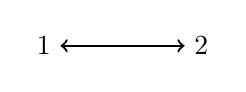
\begin{tikzpicture}
\node (atom4) at (0,0) {1};
\node (atom5) at (2,0) {2};
\draw[<->, thick] (atom4)--(atom5);
\end{tikzpicture}
\end{center}}
\end{multicols}


\problempart 
\label{pr.justifyFOLproof}
The following three proofs are missing their citations (rule and line numbers). Add them, to turn them into bona fide proofs. 
\begin{multicols}{2}
\begin{proof}
\hypo{p1}{\forall x\exists y(Rxy \eor Ryx)}
\hypo{p2}{\forall x\enot Rmx}
\have{3}{\exists y(Rmy \eor Rym)}\Ae{p1}
	\open
		\hypo{a1}{Rma \eor Ram}
		\have{a2}{\enot Rma}\Ae{p2}
		\have{a3}{Ram}\ds{a1, a2}
		\have{a4}{\exists x Rxm}\Ei{a3}
	\close
\have{n}{\exists x Rxm}\Ee{3, a1-a4}
\end{proof}

\begin{proof}
\hypo{1}{\forall x(\exists yLxy \eif \forall zLzx)}
\hypo{2}{Lab}
\have{3}{\exists y Lay \eif \forall zLza}\Ae{1}
\have{4}{\exists y Lay}\Ei{2}
\have{5}{\forall z Lza}\ce{3, 4}
\have{6}{Lca}\Ae{5}
\have{7}{\exists y Lcy \eif \forall zLzc}\Ae{1}
\have{8}{\exists y Lcy}\Ei{6}
\have{9}{\forall z Lzc}\ce{7, 8}
\have{10}{Lcc}\Ae{9}
\have{11}{\forall x Lxx}\Ai{10}
\end{proof}

\begin{proof}
\hypo{a}{\forall x(Jx \eif Kx)}
\hypo{b}{\exists x\forall y Lxy}
\hypo{c}{\forall x Jx}
\open
	\hypo{2}{\forall y Lay}
	\have{3}{Laa}\Ae{2}
	\have{d}{Ja}\Ae{c}
	\have{e}{Ja \eif Ka}\Ae{a}
	\have{f}{Ka}\ce{e, d}
	\have{4}{Ka \eand Laa}\ai{f, 3}
	\have{5}{\exists x(Kx \eand Lxx)}\Ei{4}
\close
\have{j}{\exists x(Kx \eand Lxx)}\Ee{b, 2-5}
\end{proof}
\end{multicols}


\problempart
\label{pr.BarbaraEtc.proof1}
In \S\ref{s:MoreMonadic} problem part A, we considered fifteen syllogistic figures of Aristotelian logic. Provide proofs for each of the argument forms. NB: You will find it \emph{much} easier if you symbolize (for example) `No F is G' as `$\forall x (Fx \eif \enot Gx)$'.
\\\myanswer{I shall prove the four Figure I syllogisms; the rest are \emph{extremely} similar.
\begin{multicols}{2}
\noindent \textbf{Barbara}
\begin{proof}
\hypo{gf}{\forall x (Gx \eif Fx)}
\hypo{hg}{\forall x (Hx \eif Gx)}
\have{gafa}{Ga \eif Fa}\Ae{gf}
\have{haga}{Ha \eif Ga}\Ae{hg}
\open
	\hypo{ha}{Ha}
	\have{ga}{Ga}\ce{haga, ha}
	\have{fa}{Fa}\ce{gafa, ga}
\close
\have{hafa}{Ha \eif Fa}\ci{ha-fa}
\have{con}{\forall x (Hx \eif Fx)}\Ai{hafa}
\end{proof}
\vfill
\noindent\textbf{Celerant} is exactly as Barbara, replacing `$F$' with `$\enot F$' throughout.
\columnbreak
\\\textbf{Ferio} 
\begin{proof}
\hypo{gnf}{\forall x (Gx \eif \enot Fx)}
\hypo{hg}{\exists x (Hx \eand  Gx)}
\open
	\hypo{haga}{Ha \eand Ga}
	\have{ha}{Ha}\ae{haga}
	\have{ga}{Ga}\ae{haga}
	\have{ganfa}{Ga \eif \enot Fa}\Ae{gnf}
	\have{nfa}{\enot Fa}\ce{ganfa, ga}
	\have{hanfa}{Ha \eand \enot Fa}\ai{ha, nfa}
	\have{hnf}{\exists x (Hx \eand \enot Fx)}\Ei{hanfa}
\close
\have{con}{\exists x (Hx \eand \enot Fx)}\Ee{hg, haga-hnf}
\end{proof}
\\\textbf{Darii} is exactly as Ferio, replacing `$\enot F$' with `$F$' throughout.\end{multicols}}

\

\problempart
\label{pr.BarbaraEtc.proof2}
Aristotle and his successors identified other syllogistic forms which depended upon `existential import'. Symbolize each of the following argument forms in FOL and offer proofs.
\begin{ebullet}
\newpage	\item \textbf{Barbari.} Something is H. All G are F. All H are G. So: Some H is F
	\\\myanswer{$\exists x Hx, \forall x(Gx \eif Fx), \forall x (Hx \eif Gx) \therefore \exists x (Hx \eand Fx)$
\begin{proof}
\hypo{imp}{\exists x Hx}
\hypo{gf}{\forall x (Gx \eif Fx)}
\hypo{hg}{\forall x (Hx \eif Gx)}
\open
	\hypo{ha}{Ha}
	\have{haga}{Ha \eif Ga}\Ae{hg}
	\have{ga}{Ga}\ce{haga, ha}
	\have{gafa}{Ga \eif Fa}\Ae{gf}
	\have{fa}{Fa}\ce{gafa, ga}
	\have{hafa}{Ha \eand Fa}\ai{ha, fa}
	\have{hf}{\exists x (Hx \eand Fx)}\Ei{hafa}
\close
\have{con}{\exists x (Hx \eand Fx)}\Ee{imp, ha-hf}
\end{proof}}
	
	\item \textbf{Celaront.} Something is H. No G are F. All H are G. So: Some H is not F
	\\\myanswer{$\exists x Hx, \forall x(Gx \eif \enot Fx), \forall x (Hx \eif Gx) \therefore \exists x (Hx \eand \enot Fx)$
\\	Proof is exactly as for Barbari, replacing `$F$' with `$\enot F$' throughout.}
	\item \textbf{Cesaro.} Something is H. No F are G. All H are G. So: Some H is not F.
	\\\myanswer{$\exists x Hx, \forall x(Fx \eif \enot Gx), \forall x (Hx \eif Gx) \therefore \exists x (Hx \eand \enot Fx)$
\begin{proof}
\hypo{imp}{\exists x Hx}
\hypo{fg}{\forall x (Fx \eif \enot Gx)}
\hypo{hng}{\forall x (Hx \eif  Gx)}
\open
	\hypo{ha}{Ha}
	\have{hanga}{Ha \eif Ga}\Ae{hng}
	\have{nga}{Ga}\ce{hanga, ha}
	\have{faga}{Fa \eif \enot Ga}\Ae{fg}
	\open
		\hypo{fa}{Fa}
		\have{ga}{\enot Ga}\ce{faga, fa}
		\have{red}{\ered}\ri{nga, ga}
	\close
	\have{nfa}{\enot Fa}\ni{fa-red}
	\have{hanfa}{Ha \eand \enot Fa}\ai{ha, nfa}
	\have{hnf}{\exists x (Hx \eand \enot Fx)}\Ei{hanfa}
\close
\have{con}{\exists x (Hx \eand \enot Fx)}\Ee{imp, ha-hnf}
\end{proof}
}
\newpage	\item \textbf{Camestros.} Something is H. All F are G. No H are G. So: Some H is not F.
	\\\myanswer{$\exists x Hx, \forall x(Fx \eif Gx), \forall x (Hx \eif \enot Gx) \therefore \exists x (Hx \eand \enot Fx)$
\begin{proof}
\hypo{imp}{\exists x Hx}
\hypo{fg}{\forall x (Fx \eif Gx)}
\hypo{hng}{\forall x (Hx \eif \enot Gx)}
\open
	\hypo{ha}{Ha}
	\have{hanga}{Ha \eif \enot Ga}\Ae{hng}
	\have{nga}{\enot Ga}\ce{hanga, ha}
	\have{faga}{Fa \eif Ga}\Ae{fg}
	\have{nfa}{\enot Fa}\mt{faga, nga}
	\have{hanfa}{Ha \eand \enot Fa}\ai{ha, nfa}
	\have{hnf}{\exists x (Hx \eand \enot Fx)}\Ei{hanfa}
\close
\have{con}{\exists x (Hx \eand \enot Fx)}\Ee{imp, ha-hnf}
\end{proof}}

	\item \textbf{Felapton.} Something is G. No G are F. All G are H. So: Some H is not F.
	\\\myanswer{$\exists x Gx, \forall x (Gx \eif \enot Fx), \forall x(Gx \eif Hx) \therefore \exists x (Hx \eand \enot Fx)$
\begin{proof}
\hypo{imp}{\exists x Gx}
\hypo{gnf}{\forall x (Gx \eif \enot Fx)}
\hypo{gh}{\forall x (Gx \eif Hx)}
\open
	\hypo{ga}{Ga}
	\have{gaha}{Ga \eif Ha}\Ae{gh}
	\have{ha}{Ha}\ce{gaha, ga}
	\have{ganfa}{Ga \eif \enot Fa}\Ae{gnf}
	\have{nfa}{\enot Fa}\ce{ganfa, ga}
	\have{hanfa}{Ha \eand \enot Fa}\ai{ha, nfa}
	\have{hnf}{\exists x (Hx \eand \enot Fx)}\Ei{hanfa}
\close
\have{con}{\exists x (Hx \eand Fx)}\Ee{imp, ga-hnf}
\end{proof}}
	\item \textbf{Darapti.} Something is G. All G are F. All G are H. So: Some H is F.
	\\\myanswer{$\exists x Gx, \forall x (Gx \eif Fx), \forall x(Gx \eif Hx) \therefore \exists x (Hx \eand Fx)$\\
	Proof is exactly as for Felapton, replacing `$\enot F$' with `$F$' throughout.}

\newpage	\item \textbf{Calemos.} Something is H. All F are G. No G are H. So: Some H is not F.
	\\\myanswer{$\exists x Hx, \forall x(Fx \eif Gx), \forall x(Gx \eif \enot Hx) \therefore \exists x (Hx \eand \enot Fx)$
\begin{proof}
\hypo{imp}{\exists x Hx}
\hypo{fg}{\forall x (Fx \eif Gx)}
\hypo{gnh}{\forall x (Gx \eif \enot Hx)}
\open
	\hypo{ha}{Ha}
	\have{ganha}{Ga \eif \enot Ha}\Ae{gnh}
	\open
		\hypo{ga}{Ga}
		\have{nha}{\enot Ha}\ce{ganha, ga}
		\have{red}{\ered}\ri{ha, nha}
	\close
	\have{nga}{\enot Ga}\ni{ga-red}
	\have{faga}{Fa \eif Ga}\Ae{fg}
	\have{nfa}{\enot Fa}\mt{faga, nga}
	\have{hanfa}{Ha \eand \enot Fa}\ai{ha, nfa}
	\have{hnf}{\exists x (Hx \eand Fx)}\Ei{hanfa}
\close
\have{con}{\exists x (Hx \eand Fx)}\Ee{imp, ha-hnf}
\end{proof}}
	
	\item \textbf{Fesapo.} Something is G. No F is G. All G are H. So: Some H is not F.
	\\\myanswer{$\exists x Gx, \forall x(Fx \eif \enot Gx), \forall x(Gx \eif Hx) \therefore \exists x (Hx \eand \enot Fx)$
	\begin{proof}
\hypo{imp}{\exists x Gx}
\hypo{fng}{\forall x (Fx \eif \enot Gx)}
\hypo{gh}{\forall x (Gx \eif Hx)}
\open
	\hypo{ga}{Ga}
	\have{gaha}{Ga \eif  Ha}\Ae{gh}
	\have{ha}{Ha}\ce{gaha, ga}
	\have{fanga}{Fa \eif \enot Ga}\Ae{fng}
	\open
		\hypo{fa}{Fa}
		\have{nga}{\enot Ga}\ce{fanga, fa}
		\have{red}{\ered}\ri{ga, nga}
	\close
	\have{nfa}{\enot Fa}\ni{fa-red}
	\have{hanfa}{Ha \eand \enot Fa}\ai{ha, nfa}
	\have{hnf}{\exists x (Hx \eand Fx)}\Ei{hanfa}
\close
\have{con}{\exists x (Hx \eand Fx)}\Ee{imp, ga-hnf}
\end{proof}}

\newpage	\item \textbf{Bamalip.} Something is F. All F are G. All G are H. So: Some H are F.
	\\\myanswer{$\exists x Fx, \forall x(Fx \eif Gx), \forall x(Gx \eif Hx) \therefore \exists x (Hx \eand Fx)$
\begin{proof}
\hypo{imp}{\exists x Fx}
\hypo{fg}{\forall x (Fx \eif Gx)}
\hypo{gh}{\forall x (Gx \eif Hx)}
\open
	\hypo{fa}{Fa}
	\have{faga}{Fa \eif Ga}\Ae{fg}
	\have{ga}{Ga}\ce{faga, fa}
	\have{gaha}{Ga \eif Ha}\Ae{gh}
	\have{ha}{Ha}\ce{gaha, ga}
	\have{hafa}{Ha \eand Fa}\ai{ha, fa}
	\have{hf}{\exists x (Hx \eand Fx)}\Ei{hafa}
\close
\have{con}{\exists x (Hx \eand Fx)}\Ee{imp, fa-hf}
\end{proof}}
\end{ebullet}

\problempart
\label{pr.someFOLproofs}
Provide a proof of each claim.
\begin{earg}
\item $\proves \forall x Fx \eor \enot \forall x Fx$
\myanswer{\begin{proof}
\open
	\hypo{Af}{\forall x Fx}
	\have{con}{\forall x Fx \eor \enot \forall x Fx}\oi{Af}
\close
\open
	\hypo{nAf}{\enot \forall x Fx}
	\have{con1}{\forall x Fx \eor \enot \forall x Fx}\oi{nAf}
\close
\have{con2}{\forall x Fx \eor \enot \forall x Fx}\tnd{Af-con, nAf-con1}
\end{proof}}
\item $\proves\forall z (Pz \eor \enot Pz)$
\myanswer{\begin{proof}
\open
	\hypo{Pa}{Pa}
	\have{con}{Pa \eor \enot Pa}\oi{Pa}
\close
\open
	\hypo{nPa}{\enot Pa}
	\have{con1}{Pa \eor \enot Pa}\oi{nPa}
\close
\have{con2}{Pa \eor \enot Pa}\tnd{Pa-con, nPa-con1}
\have{done}{\forall x(Px \eor \enot Px)}\Ai{con2}
\end{proof}}

\item $\forall x(Ax\eif Bx), \exists x Ax \proves \exists x Bx$
\myanswer{\begin{proof}
\hypo{Aab}{\forall x (Ax \eif Bx)}
\hypo{Ea}{\exists x Ax}
\open
	\hypo{a}{Aa}
	\have{ab}{Aa \eif Ba}\Ae{Aab}
	\have{b}{Ba}\ce{ab, a}
	\have{Eb}{\exists x Bx}\Ei{b}
\close
\have{Eb1}{\exists x Bx}\Ee{Ea, a-Eb}
\end{proof}}

\newpage\item $\forall x(Mx \eiff Nx), Ma\eand\exists x Rxa\proves \exists x Nx$
\myanswer{\begin{proof}
\hypo{Amn}{\forall x (Mx \eiff Nx)}
\hypo{mEr}{Ma \eand \exists x Rxa}
\have{m}{Ma}\ae{mEr}
\have{mn}{Ma \eiff Na}\Ae{Amn}
\have{n}{Na}\be{mn, m}
\have{En}{\exists x Nx}\Ei{n}
\end{proof}}

\item $\forall x \forall y Gxy\proves\exists x Gxx$
\myanswer{\begin{proof}
\hypo{AAg}{\forall x \forall y Gxy}
\have{Ag}{\forall y Gay}\Ae{AAg}
\have{g}{Gaa}\Ae{Ag}
\have{Eg}{\exists x Gxx}\Ei{g}
\end{proof}}

\item $\proves\forall x Rxx\eif \exists x \exists y Rxy$
\myanswer{\begin{proof}
\open
	\hypo{Ar}{\forall x Rxx}
	\have{r}{Raa}\Ae{Ar}
	\have{Er}{\exists y Ray}\Ei{r}
	\have{EEr}{\exists x \exists y Rxy}\Ei{Er}
\close
\have{ArEEr}{\forall x Rxx \eif \exists x \exists y Rxy}\ci{Ar-EEr}
\end{proof}}

\item $\proves\forall y \exists x (Qy \eif Qx)$
\myanswer{\begin{proof}
\open
	\hypo{q}{Qa}
	\have{q1}{Qa}\by{R}{q}
\close
\have{qq}{Qa \eif Qa}\ci{q-q1}
\have{Eqq}{\exists x(Qa \eif Qx)}\Ei{qq}
\have{AEqq}{\forall y \exists x(Qy \eif Qx)}\Ai{Eqq}
\end{proof}}


\item $Na \eif \forall x(Mx \eiff Ma), Ma, \enot Mb\proves \enot Na$
\myanswer{\begin{proof}
\hypo{nAmm}{Na \eif \forall x(Mx \eiff Ma)}
\hypo{m}{Ma}
\hypo{nm}{\enot Mb}
\open
	\hypo{n}{Na}
	\have{Amm}{\forall x (Mx \eiff Ma)}\ce{nAmm, n}
	\have{mm}{Mb \eiff Ma}\Ae{Amm}
	\have{mb}{Mb}\be{mm, m}
	\have{red}{\ered}\ri{mb, nm}
\close
\have{nn}{\enot Na}\ni{n-red}
\end{proof}}

\newpage\item $\forall x \forall y (Gxy \eif Gyx) \proves \forall x\forall y (Gxy \eiff Gyx)$
\myanswer{\begin{proof}
\hypo{AAgg}{\forall x \forall y(Gxy \eif Gyx)}
\open
	\hypo{gab}{Gab}
	\have{Agg}{\forall y(Gay \eif Gya)}\Ae{AAgg}
	\have{gg}{Gab \eif Gba}\Ae{Agg}
	\have{gba}{Gba}\ce{gg, gab}
\close
\open
	\hypo{gba1}{Gba}
	\have{Agg1}{\forall y(Gby \eif Gyb)}\Ae{AAgg}
	\have{gg1}{Gba \eif Gab}\Ae{Agg1}
	\have{gab1}{Gab}\ce{gg1, gba1}
\close
\have{bi}{Gab \eiff Gba}\bi{gab-gba, gba1-gab1}
\have{Abi}{\forall y(Gay \eiff Gya)}\Ai{bi}
\have{AAbi}{\forall x \forall y (Gxy \eiff Gyx)}\Ai{Abi}
\end{proof}}

\item $\forall x(\enot Mx \eor Ljx), \forall x(Bx\eif Ljx), \forall x(Mx\eor Bx)\proves \forall xLjx$
\myanswer{\begin{proof}
\hypo{Anmlj}{\forall x (\enot Mx \eor Ljx)}
\hypo{Ablj}{\forall x (Bx \eif Ljx)}
\hypo{Amb}{\forall x (Mx \eor Bx)}
\have{nmlj}{\enot Ma \eor Ljx}\Ae{Anmlj}
\have{blj}{Ba \eif Lja}\Ae{Ablj}
\have{mb}{Ma \eor Ba}\Ae{Amb}
\open
	\hypo{nm}{\enot Ma}
	\have{b}{Ba}\ds{mb, nm}
	\have{lj}{Lja}\ce{blj, b}
\close
\open
	\hypo{lj1}{Lja}
	\have{lj2}{Lja}\by{R}{lj1}
\close
\have{lj3}{Lja}\oe{nmlj, nm-lj, lj1-lj2}
\have{Alj}{\forall x Ljx}\Ai{lj3}
\end{proof}}
\end{earg}

\solutions
\problempart
\label{pr.likes}
Write a symbolization key for the following argument, symbolize it, and prove it:
\begin{quote}
There is someone who likes everyone who likes everyone that she likes. Therefore, there is someone who likes herself.
\end{quote}
\myanswer{Symbolization key:
\begin{ekey}
\item[\text{domain}] all people
\item[Lxy] \gap{x} likes \gap{y}
\end{ekey}
$\exists x \forall y(\forall z(Lxz \eif Lyz) \eif Lxy) \therefore \exists x  Lxx$
\begin{proof}
\hypo{1}{\exists x\forall y(\forall z(Lxz \eif Lyz) \eif Lxy)}
\open
	\hypo{a}{\forall y(\forall z(Laz \eif Lyz) \eif Lay)}
	\have{b}{\forall z(Laz \eif Laz) \eif Laa} \Ae{a}
	\open
		\hypo{lac}{Lac}
		\have{lac1}{Lac}\by{R}{lac}
	\close
	\have{laclac}{Lac \eif Lac}\ci{lac-lac1}
	\have{Alaz}{\forall z (Laz \eif Laz)}\Ai{laclac}
	\have{laa}{Laa}\ce{b, Alaz}
	\have{El}{\exists x Lxx}\Ei{laa}
\close
\have{n}{\exists x Lxx} \Ee{1, a--El}
\end{proof}}

\problempart
Show that each pair of sentences is provably equivalent.
\begin{earg}
\item $\forall x (Ax\eif \enot Bx)$, $\enot\exists x(Ax \eand Bx)$
\item $\forall x (\enot Ax\eif Bd)$, $\forall x Ax \eor Bd$
\item $\exists x Px \eif Qc$, $\forall x (Px \eif Qc)$
\end{earg}


\solutions
\problempart
\label{pr.FOLequivornot}
For each of the following pairs of sentences: If they are provably equivalent, give proofs to show this. If they are not, construct an interpretation to show that they are not logically equivalent.
\begin{earg}
\item $\forall x Px \eif Qc, \forall x (Px \eif Qc)$ \hfill \myanswer{Not logically equivalent}
\\\myanswer{Counter-interpretation: let the domain be the numbers $1$ and $2$. Let `$c$' name $1$. Let `$Px$' be true of and only of $1$. Let `$Qx$' be true of, and only of, $2$.}
\item $\forall x\forall y \forall z Bxyz, \forall x Bxxx$\hfill \myanswer{Not logically equivalent}
\\\myanswer{Counter-interpretation: let the domain be the numbers $1$ and $2$. Let `$Bxyz$' be true of, and only of, \ntuple{1,1,1} and \ntuple{2,2,2}.}
\item $\forall x\forall y Dxy, \forall y\forall x Dxy$ \hfill \myanswer{Provably equivalent\begin{multicols}{2}
\begin{proof}
\hypo{AAd}{\forall x \forall y Dxy}
\have{Ad}{\forall y Day}\Ae{AAd}
\have{A}{Dab}\Ae{Ad}
\have{Ad1}{\forall x Dxb}\Ai{A}
\have{AAd1}{\forall y \forall x Dxy}\Ai{Ad1}
\end{proof}
\begin{proof}
\hypo{AAd}{\forall y \forall x Dxy}
\have{Ad}{\forall x Dxa}\Ae{AAd}
\have{A}{Dba}\Ae{Ad}
\have{Ad1}{\forall y Dby}\Ai{A}
\have{AAd1}{\forall x \forall y Dxy}\Ai{Ad1}
\end{proof}
\end{multicols}}
\item $\exists x\forall y Dxy, \forall y\exists x Dxy$ \hfill \myanswer{Not logically equivalent}
\\\myanswer{Counter-interpretation: let the domain be the numbers $1$ and $2$. Let `$Dxy$' hold of and only of \ntuple{1,2} and \ntuple{2,1}. This is depicted thus:
\begin{center}
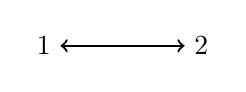
\begin{tikzpicture}
\node (atom4) at (0,0) {1};
\node (atom5) at (2,0) {2};
\draw[<->, thick] (atom4)--(atom5);
\end{tikzpicture}
\end{center}}
\item $\forall x (Rca \eiff Rxa), Rca \eiff \forall x Rxa$ \hfill \myanswer{Not logically equivalent}
\\\myanswer{Counter-interpretation, consider the following diagram, allowing `$a$' to name 1 and `$c$' to name 2:
\begin{center}
\begin{tikzpicture}
\node (atom4) at (0,0) {1};
\node (atom5) at (2,0) {2};
\draw[->, thick] (atom4)+(-0.15,0.15) arc (-330:-30:.3); 
%\draw[->, thick] (atom5)+(0.15,-0.15) arc (-150:150:.3); 
%\draw[<->, thick] (atom4)--(atom5);
\end{tikzpicture}
\end{center}}
\end{earg}

\solutions
\problempart
\label{pr.FOLvalidornot}
For each of the following arguments: If it is valid in FOL, give a proof. If it is invalid, construct an interpretation to show that it is invalid.
\begin{earg}
\item $\exists y\forall x Rxy \therefore \forall x\exists y Rxy$ \hfill \myanswer{Valid
\begin{proof}
\hypo{EAr}{\exists y \forall x Rxy}
\open
	\hypo{Ar}{\forall x Rxa}
	\have{r}{Rba}\Ae{Ar}
	\have{Er}{\exists y Rby}\Ei{r}
\close
\have{Er1}{\exists y Rby}\Ee{EAr, Ar-Er}
\have{AEr}{\forall x \exists y Rxy}\Ai{Er1}
\end{proof}}
\item $\exists x(Px \eand \enot Qx) \therefore \forall x(Px \eif \enot Qx)$ \hfill \myanswer{Not valid
\\Counter interpretation: let the domain be the numbers $1$ and $2$. Let `$Px$' be true of everything in the domain. Let `$Qx$' be true of, and only of, $2$.}
\item $\forall x(Sx \eif Ta), Sd \therefore Ta$ \hfill \myanswer{Valid
\begin{proof}
\hypo{Ast}{\forall x (Sx \eif Ta)}
\hypo{s}{Sd}
\have{st}{Sd \eif Ta}\Ae{Ast}
\have{t}{Ta}\ce{st, s}
\end{proof}}
\item $\forall x(Ax\eif Bx), \forall x(Bx \eif Cx) \therefore \forall x(Ax \eif Cx)$ \hfill \myanswer{Valid
\begin{proof}
\hypo{Aab}{\forall x (Ax \eif Bx)}
\hypo{Abc}{\forall x (Bx \eif Cx)}
\have{ab}{Aa \eif Ba}\Ae{Aab}
\have{bc}{Ba \eif Ca}\Ae{Abc}
\open
	\hypo{a}{Aa}
	\have{b}{Ba}\ce{ab, a}
	\have{c}{Ca}\ce{bc, b}
\close
\have{ac}{Aa \eif Ca}\ci{a-c}
\have{Aac}{\forall x (Ax \eif Cx)}\Ai{ac}
\end{proof}}
\item $\exists x(Dx \eor Ex), \forall x(Dx \eif Fx) \therefore \exists x(Dx \eand Fx)$ \hfill \myanswer{Invalid\\
Counter-interpretation: let the domain be the number $1$ . Let `$Dx$' hold of nothing. Let both `$Ex$' and `$Fx$' hold of everything.}
\item $\forall x\forall y(Rxy \eor Ryx) \therefore Rjj$ \hfill \myanswer{Valid
\begin{proof}
\hypo{AArr}{\forall x \forall y (Rxy \eor Ryx)}
\have{Arr}{\forall y (Rjy \eor Ryj)}\Ae{AArr}
\have{rr}{Rjj \eor Rjj}\Ae{Arr}
\open
	\hypo{r1}{Rjj}
	\have{r2}{Rjj}\by{R}{r1}
\close
\open
	\hypo{r3}{Rjj}
	\have{r4}{Rjj}\by{R}{r3}
\close
\have{r5}{Rjj}\oe{rr, r1-r2, r3-r4}
\end{proof}}

\item $\exists x\exists y(Rxy \eor Ryx) \therefore Rjj$ \hfill \myanswer{Invalid\\
Counter-interpretation: consider the following diagram, allowing `$j$' to name $2$.
\begin{center}
\begin{tikzpicture}
\node (atom4) at (0,0) {1};
\node (atom5) at (2,0) {2};
\draw[->, thick] (atom4)+(-0.15,0.15) arc (-330:-30:.3); 
%\draw[->, thick] (atom5)+(0.15,-0.15) arc (-150:150:.3); 
%\draw[<->, thick] (atom4)--(atom5);
\end{tikzpicture}
\end{center}}
\item $\forall x Px \eif \forall x Qx, \exists x \enot Px \therefore \exists x \enot Qx$ \hfill \myanswer{Invalid\\
Counter-interpretation: let the domain be the number $1$. Let `$Px$' be true of nothing. Let `$Qx$' be true of everything.}
\end{earg}


\chapter{Conversion of quantifiers}\setcounter{ProbPart}{0}
\problempart
Show in each case that the sentences are provably inconsistent:
\begin{earg}
\item $Sa\eif Tm, Tm \eif Sa, Tm \eand \enot Sa$
\myanswer{\begin{proof}
\hypo{st}{Sa \eif Tm}
\hypo{ts}{Tm \eif Sa}
\hypo{tns}{Tm \eand \enot Sa}
\have{t}{Tm}\ae{tns}
\have{ns}{\enot Sa}\ae{tns}
\have{s}{Sa}\ce{ts, t}
\have{red}{\ered}\ri{ns,s}
\end{proof}}
\item $\enot\exists x Rxa, \forall x \forall y Ryx$
\myanswer{\begin{proof}
\hypo{nEr}{\enot \exists x Rxa}
\hypo{AAr}{\forall x \forall y Ryx}
\have{Anr}{\forall x \enot Rxa}\cq{nEr}
\have{nr}{\enot Rba}\Ae{Anr}
\have{Ar}{\forall y Rya}\Ae{AAr}
\have{r}{Rba}\Ae{Ar}
\have{red}{\ered}\ri{r, nr}
\end{proof}}
\item $\enot\exists x \exists y Lxy, Laa$
\myanswer{\begin{proof}
\hypo{nEEl}{\enot \exists x \exists y Lxy}
\hypo{l}{Laa}
\have{AnEl}{\forall x \enot \exists y Lxy}\cq{nEEl}
\have{nEl}{\enot \exists y Lay}\Ae{AnEl}
\have{Anl}{\forall y \enot Lay}\cq{nEl}
\have{n}{\enot Laa}\Ae{Anl}
\have{red}{\ered}\ri{l,n}
\end{proof}}
\item $\forall x(Px \eif Qx), \forall z(Pz \eif Rz), \forall y Py, \enot Qa \eand \enot Rb$
\myanswer{\begin{proof}
\hypo{Apq}{\forall x(Px \eif Qx)}
\hypo{Apr}{\forall z(Pz \eif Rz)}
\hypo{Ap}{\forall y Py}
\hypo{nqnr}{\enot Qa \eand \enot Rb}
\have{nq}{\enot Qa}\ae{nqnr}
\have{pq}{Pa \eif Qa}\Ae{Apq}
\have{np}{\enot Pa}\mt{pq, nq}
\have{p}{Pa}\Ae{Ap}
\have{red}{\ered}\ri{p,np}
\end{proof}}
\end{earg}

\problempart
Show that each pair of sentences is provably equivalent: %TB: Again, have to do some manual numbering to make the multicols have enough space.

\

1.  $\forall x (Ax\eif \enot Bx), \enot\exists x(Ax \eand Bx)$
\myanswer{\begin{multicols}{2}
\begin{proof}
\hypo{Aanb}{\forall x (Ax \eif \enot Bx)}
\open
	\hypo{Eab}{\exists x (Ax \eand Bx)}
	\open
		\hypo{ab}{Aa \eand Ba}
		\have{a}{Aa}\ae{ab}
		\have{b}{Ba}\ae{ab}
		\have{anb}{Aa \eif \enot Ba}\Ae{Aanb}
		\have{nb}{\enot Ba}\ce{anb, a}
		\have{red}{\ered}\ri{b, nb}
	\close
	\have{red1}{\ered}\Ee{Eab, ab-red}
	\close
\have{nEab}{\enot \exists x(Ax \eand Bx)}\ni{Eab-red1}
\end{proof}
\begin{proof}
\hypo{nEab}{\enot \exists x(Ax \eand Bx)}
\have{Anab}{\forall x\enot(Ax \eand Bx)}\cq{nEab}
\have{nab}{\enot (Aa \eand Ba)}\Ae{Anab}
\open
	\hypo{a}{Aa}
	\open
		\hypo{b}{Ba}
		\have{ab}{Aa \eand Ba}\ai{a,b}
		\have{red}{\ered}\ri{ab,nab}
	\close
	\have{nb}{\enot Ba}\ni{b-red}
\close
\have{anb}{Aa \eif \enot Ba}\ci{a-nb}
\have{Aanb}{\forall x (Ax \eif \enot Bx)}\Ai{anb}		
\end{proof}
\end{multicols}}
2. $\forall x (\enot Ax\eif Bd), \forall x Ax \eor Bd$
\myanswer{\begin{multicols}{2}
\begin{proof}
\hypo{Anab}{\forall x(\enot Ax \eif Bd)}
\have{nab}{\enot Aa \eif Bd}\Ae{Anab}
\open
	\hypo{b}{Bd}
	\have{Aab}{\forall x Ax \eor Bd}\oi{ab}
\close
\open
	\hypo{nb}{\enot Bd}
	\have{nna}{\enot \enot Aa}\mt{nab, nb}
	\have{a}{Aa}\dne{nna}
	\have{Aa}{\forall x Ax}\Ae{a}
	\have{Aab1}{\forall x Ax \eor Bd}\oi{Aa}
\close
\have{Aab2}{\forall xAx \eor Bd}\tnd{b-Aab, nb-Aab1}
\end{proof}
\begin{proof}
\hypo{Aab}{\forall x Ax \eor Bd}
\open
	\hypo{na}{\enot Aa}
	\open
		\hypo{Aa}{\forall x Ax}
		\have{a}{Aa}\Ae{Aa}
		\have{red}{\ered}\ri{a, na}
	\close
	\have{nAa}{\enot \forall x Ax}\ni{Aa-red}
	\have{b}{Bd}\ds{Aab, nAa}
\close
\have{nab}{\enot Aa \eif Bd}\ci{na-b}
\have{Anab}{\forall x (Ax \eif Bd)}\Ai{nab}
\end{proof}
\end{multicols}}


\problempart
In \S\ref{s:MoreMonadic}, we considered what happens when we move quantifiers `across' various logical operators. Show that each pair of sentences is provably equivalent: %TB: Again, manual line numbering to give multicols enough space.

\

1.  $\forall x (Fx \eand Ga), \forall x Fx \eand Ga$ 
\myanswer{
\begin{multicols}{2}
\begin{proof}
\hypo{Afg}{\forall x (Fx \eand Ga)}
\have{fg}{Fb \eand Ga}\Ae{Afg}
\have{f}{Fb}\ae{fg}
\have{g}{Ga}\ae{ga}
\have{Af}{\forall x Fx}\Ai{f}
\have{Afg1}{\forall x Fx \eand Ga}\ai{Af, g}
\end{proof}
\begin{proof}
\hypo{Afg}{\forall x Fx \eand Ga}
\have{Af}{\forall x Fx}\ae{Afg}
\have{g}{Ga}\ae{Afg}
\have{f}{Fb}\Ae{Af}
\have{fg}{Fb \eand Ga}\ai{f, g}
\have{Afg1}{\forall x (Fx \eand Ga)}\Ai{fg}
\end{proof}
\end{multicols}}
2. $\exists x (Fx \eor Ga), \exists x Fx \eor Ga$
\myanswer{
\begin{multicols}{2}
\begin{proof}
\hypo{Efg}{\exists x (Fx \eor Ga)}
\open
	\hypo{fg}{Fb \eor Ga}
	\open
		\hypo{f}{Fb}
		\have{Ef}{\exists x Fx}\Ei{f}
		\have{Efg1}{\exists x Fx \eor Ga}\oi{Ef}
	\close
	\open
		\hypo{g}{Ga}
		\have{Efg2}{\exists x Fx \eor Ga}\oi{g}
	\close		
	\have{Efg3}{\exists x Fx \eor Ga}\oe{fg, f-Efg1, g-Efg2}
\close
\have{Efg4}{\exists x Fx \eor Ga}\Ee{Efg, fg-Efg3}
\end{proof}
\begin{proof}
\hypo{Efg}{\exists x Fx \eor Ga}
\open
	\hypo{Ef}{\exists x Fx}
	\open
		\hypo{f}{Fb}
		\have{fg}{Fb \eor Ga}\oi{f}
		\have{Efg1}{\exists x (Fx \eor Ga)}\Ei{fg}
	\close
	\have{Efg2}{\exists x (Fx \eor Ga)}\Ee{Ef, f-Efg1}
\close
\open
	\hypo{g}{Ga}
	\have{fbg}{Fb \eor Ga}\oi{g}
	\have{Efg3}{\exists x (Fx \eor Ga)}\Ei{fbg}
\close
\have{Efg4}{\exists x (Fx \eor Ga)}\oe{Efg, Ef-Efg2, g-Efg3}
\end{proof}
\end{multicols}}
3. $\forall x(Ga \eif Fx), Ga \eif \forall x Fx$
\myanswer{\begin{multicols}{2}
\begin{proof}
\hypo{Agf}{\forall x(Ga \eif Fx)}
\have{gf}{Ga \eif Fb}\Ae{Agf}
\open
	\hypo{g}{Ga}
	\have{f}{Fb}\ce{gf, g}
	\have{Af}{\forall x Fx}\Ai{f}
\close
\have{gAf}{Ga \eif \forall x Fx}\ci{g-Af}
\end{proof}
\begin{proof}
\hypo{gAf}{Ga \eif \forall x Fx}
\open
	\hypo{g}{Ga}
	\have{Af}{\forall x Fx}\ce{gAf, g}
	\have{f}{Fb}\Ae{Af}
\close
\have{gf}{Ga \eif Fb}\ci{g-f}
\have{Agf}{\forall x (Ga \eif Fx)}\Ai{gf}
\end{proof}
\end{multicols}}

4. $\forall x(Fx \eif Ga), \exists x Fx \eif Ga$
\myanswer{\begin{multicols}{2}
\begin{proof}
\hypo{Afg}{\forall x(Fx \eif Ga)}
\open
	\hypo{Ef}{\exists x Fx}
	\open
		\hypo{f}{Fb}
		\have{fg}{Fb \eif Ga}\Ae{Afg}
		\have{g}{Ga}\ce{fg, f}
	\close
	\have{g1}{Ga}\Ee{Ef, f-g}
\close
\have{Efg}{\exists x Fx \eif Ga}\ci{Ef-g1}	
\end{proof}
\begin{proof}
\hypo{Efg}{\exists x Fx \eif Ga}
\open
	\hypo{f}{Fb}
	\have{Ef}{\exists x Fx}\Ei{f}
	\have{g}{Ga}\ce{Efg, Ef}
\close
\have{fg}{Fb \eif Ga}\ci{f-g}
\have{Afg}{\forall x(Fx \eif Ga)}\Ai{fg}	
\end{proof}
\end{multicols}}
5. $\exists x(Ga \eif Fx), Ga \eif \exists x Fx$
\myanswer{\begin{multicols}{2}
\begin{proof}
\hypo{Egf}{\exists x(Ga \eif Fx)}
\open
	\hypo{g}{Ga}
	\open
		\hypo{gf}{Ga \eif Fb}
		\have{f}{Fb}\ce{gf, g}
		\have{Ef}{\exists x Fx}\Ei{f}
	\close
	\have{Ef1}{\exists x Fx}\Ee{Egf, gf-Ef}
\close
\have{gEf}{Ga \eif \exists x Fx}\ci{g-Ef1}
\end{proof}
\begin{proof}
\hypo{gEf}{Ga \eif \exists x Fx}
\open
	\hypo{g}{Ga}
	\have{Ef}{\exists x Fx}
	\open
		\hypo{f}{Fb}
		\open
			\hypo{g1}{Ga}
			\have{f1}{Fb}\by{R}{f}
		\close
		\have{gf}{Ga \eif Fb}\ci{g1-f1}
		\have{Egf}{\exists x(Ga \eif Fx)}\Ei{gf}
	\close
	\have{Egf1}{\exists x (Ga \eif Fx)}\Ee{Ef, f-Egf}
\close
\open
	\hypo{ng}{\enot Ga}
	\open
		\hypo{g2}{Ga}
		\have{red}{\ered}\ri{g2, ng}
		\have{f2}{Fb}\re{red}
	\close
	\have{gf1}{Ga \eif Fb}\ce{g2-f2}
	\have{Egf2}{\exists x (Ga \eif Fx)}\Ei{gf1}
\close
\have{con}{\exists x (Ga \eif Fx)}\tnd{g-Egf1, ng-Egf2}
\end{proof}
\end{multicols}}

6. $\exists x(Fx \eif Ga), \forall x Fx \eif Ga$
\myanswer{\begin{multicols}{2}
\begin{proof}
\hypo{Efg}{\exists x (Fx \eif Ga)}
\open
	\hypo{Af}{\forall x Fx}
	\open
		\hypo{fg}{Fb \eif Ga}
		\have{f}{Fb}\Ae{Af}
		\have{g}{Ga}\ce{fg,f}
	\close
	\have{g1}{Ga}\Ee{Efg, fg-g}
\close
\have{Afg}{\forall x Fx \eif Ga}\ci{Af-g1}
\end{proof}
\begin{proof}
\hypo{Afg}{\forall x Fx \eif Ga}
\open
	\hypo{Af}{\forall x Fx}
	\have{g}{Ga}\ce{Afg, Af}
	\open
		\hypo{f}{Fb}
		\have{g1}{Ga}\by{R}{g}
	\close
	\have{fg}{Fb \eif Ga}\ci{f-g1}
	\have{Efg}{\exists x (Fx \eif Ga)}\Ei{fg}
\close
\open
	\hypo{nAf}{\enot \forall x Fx}
	\have{Enf}{\exists x \enot Fx}\cq{nAf}
	\open
		\hypo{nf}{\enot Fb}
		\open
			\hypo{f1}{Fb}
			\have{red}{\ered}\ri{f1, nf}
			\have{g2}{Ga}\re{red}
		\close
		\have{fg1}{Fb \eif Ga}\ci{f1-g2}
		\have{Efg1}{\exists x (Fx \eif Ga)}\Ei{fg1}
	\close
	\have{Efg2}{\exists x (Fx \eif Ga)}\Ee{Enf, nf-Efg1}
\close
\have{Efg3}{\exists x (Fx \eif Ga)}\tnd{Af-Efg, nAf-Efg2}
\end{proof}
\end{multicols}}
NB: the variable `$x$' does not occur in `$Ga$'.

When all the quantifiers occur at the beginning of a sentence, that sentence is said to be in \emph{prenex normal form}. Together with the CQ rules, these equivalences are sometimes called \emph{prenexing rules}, since they give us a means for putting any sentence into prenex normal form.

\chapter{Rules for identity}\setcounter{ProbPart}{0}
\problempart
\label{pr.identity}
Provide a proof of each claim.
\begin{earg}
\item $Pa \eor Qb, Qb \eif b=c, \enot Pa \proves Qc$
\myanswer{
\begin{proof}
\hypo{pq}{Pa \eor Qb}
\hypo{qbi}{Qb \eif b=c}
\hypo{np}{\enot Pa}
\have{q}{Qb}\ds{pq, np}
\have{i}{b=c}\ce{qbi, q}
\have{qc}{Qc}\ie{i,q}
\end{proof}}
\item $m=n \eor n=o, An \proves Am \eor Ao$
\myanswer{
\begin{proof}
\hypo{mnino}{m=n \eor n=o}
\hypo{an}{An}
\open
	\hypo{min}{m=n}
	\have{am}{Am}\ie{min, an}
	\have{amao}{Am \eor Ao}\oi{am}
\close
\open
	\hypo{nio}{n=o}
	\have{ao}{Ao}\ie{nio, ao}
	\have{amao1}{Am \eor Ao}\oi{ao}
\close
\have{amao2}{Am \eor Ao}\oe{mnino, min-amao, nio-amao1}
\end{proof}}
\item $\forall x\ x=m, Rma\proves \exists x Rxx$
\myanswer{\begin{proof}
\hypo{Axim}{\forall x\ x=m}
\hypo{rma}{Rma}
\have{aim}{a=m}\Ae{Axim}
\have{raa}{Raa}\ie{aim, rma}
\have{Erxx}{\exists x Rxx}\Ei{raa}
\end{proof}}
\item $\forall x\forall y(Rxy \eif x=y)\proves Rab \eif Rba$
\myanswer{\begin{proof}
\hypo{AArxiy}{\forall x \forall y(Rxy \eif x = y)}
\open
	\hypo{rab}{Rab}
	\have{Araiy}{\forall y(Ray \eif a = y)}\Ae{AArxiy}
	\have{raib}{Rab \eif a=b}\Ae{Araiy}
	\have{aib}{a=b}\ce{raib, rab}
	\have{raa}{Raa}\ie{aib, rab}
	\have{rba}{Rba}\ie{aib, raa}
\close
\have{rabrba}{Rab \eif Rba}\ci{rab-rba}
\end{proof}}
\item $\enot \exists x\enot x = m \proves \forall x\forall y (Px \eif Py)$
\myanswer{\begin{proof}
\hypo{nEnxim}{\enot \exists x \enot x = m}
\have{Annxim}{\forall x \enot \enot x =m}\cq{nEnxim}
\have{nnaim}{\enot \enot a = m}\Ae{Annxim}
\have{aim}{a = m}\dne{nnaim}
\have{nnbim}{\enot \enot b = m}\Ae{Annxim}
\have{bim}{b = m}\dne{nnbim}
\open
	\hypo{pa}{Pa}
	\have{pm}{Pm}\ie{nnaim, pa}
	\have{pb}{Pb}\ie{nnbim, pm}
\close
\have{papb}{Pa \eif Pb}\ci{pa-pb}
\have{Apapy}{\forall y (Pa \eif Py)}\Ai{papb}
\have{AApxpy}{\forall x\forall y (Px \eif Py)}\Ai{Apapy}
\end{proof}}
\item $\exists x Jx, \exists x \enot Jx\proves \exists x \exists y\ \enot x = y$
\myanswer{\begin{proof}
\hypo{Ej}{\exists x Jx}
\hypo{Enj}{\exists x \enot Jx}
\open
	\hypo{j}{Ja}
	\open
		\hypo{nj}{\enot Jb}
		\open
			\hypo{aib}{a=b}
			\have{jb}{Jb}\ie{aib, j}
			\have{red}{\ered}\ri{jb, nj}
		\close
		\have{naib}{\enot a = b}\ni{aib-red}
		\have{Enaiy}{\exists y \enot a = y}\Ei{naib}
		\have{EEnxiy}{\exists x \exists y \enot x = y}\Ei{Enaiy}
	\close
	\have{EEnxiy1}{\exists x \exists y \enot x = y}\Ee{Enj, nj-EEnxiy}
\close
\have{EEnxiy2}{\exists x \exists y \enot x = y}\Ee{Ej, j-EEnxiy1}
\end{proof}}

\item $\forall x(x=n \eiff Mx), \forall x(Ox \eor \enot Mx)\proves On$
\myanswer{\begin{proof}
\hypo{Axinm}{\forall x(x = n \eiff Mx)}
\hypo{Aonm}{\forall x(Ox \eor \enot Mx)}
\have{ninm}{n = n \eiff Mn}\Ae{Axinm}
\have{nin}{n=n}\ii{}
\have{m}{Mn}\be{ninm,nin}
\have{onm}{On \eor \enot Mn}\Ae{Aonm}
\open
	\hypo{no}{\enot On}
	\have{nm}{\enot Mn}\ds{onm, no}
	\have{red}{\ered}\ri{m, nm}
\close
\have{nno}{\enot\enot On}\ni{no-red}
\have{o}{On}\dne{nno}
\end{proof}}

\item $\exists x Dx, \forall x(x=p \eiff Dx)\proves Dp$
\myanswer{\begin{proof}
\hypo{Ed}{\exists x Dx}
\hypo{Axd}{\forall x(x = p \eiff Dx)}
\open
	\hypo{d}{Dc}
	\have{cipd}{c = p \eiff Dc}\Ae{Axd}
	\have{cip}{c = p}\be{cipd, d}
	\have{dp}{Dp}\ie{cip, d}
\close
\have{dp1}{Dp}\Ee{Ed, d-dp}
\end{proof}}

\item $\exists x\bigl[(Kx \eand \forall y(Ky \eif x=y)) \eand Bx\bigr], Kd\proves Bd$
\myanswer{\begin{proof}
\hypo{EkAkb}{\exists x\bigl[(Kx \eand \forall y(Ky \eif x=y) \eand Bx\bigr]}
\hypo{kd}{Kd}
\open
	\hypo{kAkb}{(Ka \eand \forall y(Ky \eif a=y)) \eand Ba}
	\have{kAk}{Ka \eand \forall y(Ky \eif a=y)}\ae{kAkb}
	\have{k}{Ka}\ae{kAk}
	\have{Ak}{\forall y (Ky \eif a = y)}\ae{kAk}
	\have{kdaid}{Kd \eif a = d}\Ae{Ak}
	\have{aid}{a = d}\ce{kdaid, kd}
	\have{b}{Ba}\ae{kAkb}
	\have{bd}{Bd}\ie{aid, b}
\close
\have{con}{Bd}\Ee{EkAkb, kAkb-bd}
\end{proof}}

\item $\proves Pa \eif \forall x(Px \eor \enot x = a)$
\myanswer{\begin{proof}
\open
	\hypo{pa}{Pa}
	\open
		\hypo{bia}{b = a}
		\have{pb}{Pb}\ie{bia, pa}
		\have{pboi}{Pb \eor \enot b = a}\oi{pb}
	\close
	\open
		\hypo{nbia}{\enot b = a}
		\have{pboi1}{Pb \eor \enot b = a}\oi{nbia}
	\close
	\have{pboi2}{Pb \eor \enot b = a}\tnd{bia-pboi, nbia-pboi1}
	\have{Apoi}{\forall x (Px \eor \enot x = a)}\Ai{pboi2}
\close
\have{con}{Pa \eif \forall x (Px \eor \enot x = a)}\ci{pa-Apoi}
\end{proof}}
\end{earg}

\problempart
Show that the following are provably equivalent:
\begin{ebullet}
\item $\exists x \bigl([Fx \eand \forall y (Fy \eif x = y)] \eand x = n\bigr)$
\item $Fn \eand \forall y (Fy \eif n= y)$
\end{ebullet}
And hence that both have a decent claim to symbolize the English sentence `Nick is the F'.
\\\myanswer{In one direction:
\begin{proof}
\hypo{prem}{\exists x \bigl([Fx \eand \forall y (Fy \eif x = y)] \eand x = n\bigr)}
\open
	\hypo{prema}{{}[Fa \eand \forall y (Fy \eif a = y)] \eand a = n}
	\have{preman}{a = n}\ae{prema}
	\have{prema1}{Fa \eand \forall y (Fy \eif a = y)}\ae{prema}
	\have{prema2}{Fa}\ae{prema1}
	\have{fn}{Fn}\ie{preman, prema2}
	\have{prema3}{\forall y (Fy \eif a = y)}\ae{prema1}
	\have{prema4}{\forall y (Fy \eif n = y)}\ie{preman, prema3}
	\have{con1}{Fn \eand \forall y (Fy \eif n= y)}\ai{fn, prema4}
\close
\have{con}{Fn \eand \forall y (Fy \eif n= y)}\Ee{prem, prema-con1}
\end{proof}\\And now in the other:
\begin{proof}
\hypo{prem}{Fn \eand \forall y (Fy \eif n= y)}
\have{nin}{n = n}\ii{}
\have{near}{{}[Fn \eand \forall y (Fy \eif n= y)] \eand n = n}\ai{prem, nin}
\have{con}{\exists x \bigl([Fx \eand \forall y (Fy \eif x = y)] \eand x = n\bigr)}\Ei{near}
\end{proof}}

\

\problempart
In \S\ref{sec.identity}, we claimed that the following are logically equivalent symbolizations of the English sentence `there is exactly one F':
\begin{ebullet}
\item $\exists x Fx \eand \forall x \forall y \bigl[(Fx \eand Fy) \eif x = y\bigr]$
\item $\exists x \bigl[Fx \eand \forall y (Fy \eif x = y)\bigr]$
\item $\exists x \forall y (Fy \eiff x = y)$
\end{ebullet}
Show that they are all provably equivalent. (\emph{Hint}: to show that three claims are provably equivalent, it suffices to show that the first proves the second, the second proves the third and the third proves the first; think about why.)\\
\myanswer{It suffices to show that the first proves the second, the second proves the third and the third proves the first, for we can then show that any of them prove any others, just by chaining the proofs together (numbering lines, where necessary. Armed with this, we start on the first proof:
\begin{proof}
\hypo{prem}{\exists x Fx \eand \forall x \forall y \bigl[(Fx \eand Fy) \eif x = y\bigr]}
\have{prem1}{\exists x Fx}\ae{prem}
\have{prem2}{\forall x \forall y \bigl[(Fx \eand Fy) \eif x = y\bigr]}\ae{prem}
\open
	\hypo{fa}{Fa}
	\have{prem2a}{\forall y \bigl[(Fa \eand Fy) \eif a = y\bigr]}\Ae{prem2}
	\have{prem2b}{(Fa \eand Fb) \eif a = b}\Ae{prem2a}
	\open
		\hypo{fb}{Fb}
		\have{fafb}{Fa \eand Fb}\ai{fa, fb}
		\have{aib}{a=b}\ce{prem2b, fafb}
	\close
	\have{fbaib}{Fb \eif a =b}\ci{fb-aib}
	\have{Afb}{\forall y(Fy \eif a =y)}\Ai{fbaib}	
	\have{cona}{Fa \eand \forall y(Fy \eif a = y))}\ai{fa, Afb}
	\have{con1}{\exists x \bigl[Fx \eand \forall y(Fy \eif x = y)\bigr]}\Ei{cona}
\close
\have{con}{\exists x \bigl[Fx \eand \forall y (Fy \eif x = y)\bigr]}\Ee{prem1, fa-con1}
\end{proof}}

\
\\\myanswer{Now for the second proof:
\begin{proof}
\hypo{prem}{\exists x \bigl[Fx \eand \forall y (Fy \eif x = y)\bigr]}
\open
	\hypo{prema}{Fa \eand \forall y (Fy \eif a = y)}
	\have{fa}{Fa}\ae{prema}
	\have{Af}{\forall y (Fy \eif a = y)}\ae{prema}
	\open
		\hypo{fb1}{Fb}
		\have{fbaib}{Fb \eif a = b}\Ae{Af}
		\have{aib1}{a = b}\ce{fbaib, fb1}
	\close
	\open
		\hypo{aib}{a = b}
		\have{fb}{Fb}\ie{aib, fa}
	\close
	\have{bic}{Fb \eiff a = b}\bi{fb1-aib1, aib-fb}
	\have{cony}{\forall y(Fy \eiff a = y)}\Ai{bic}
	\have{con1}{\exists x \forall y (Fy \eiff x = y)}\Ei{cony}
\close
\have{con}{\exists x \forall y (Fy \eiff x = y)}\Ee{prem, prema-con1}
\end{proof}}

\noindent\myanswer{And finally, the third proof:
\begin{proof}
\hypo{prem}{\exists x \forall y (Fy \eiff x = y)}
\open
	\hypo{prema}{\forall y(Fy \eiff a = y)}
	\have{premaa}{Fa \eiff a = a}\Ae{prema}
	\have{aia}{a = a}\ii{}
	\have{fa}{Fa}\be{premaa, aia}
	\have{Ef}{\exists x Fx}\Ei{fa}
	\open
		\hypo{fbfc}{Fb \eand Fc}
		\have{fb}{Fb}\ae{fbfc}
		\have{premab}{Fb \eiff a = b}\Ae{prema}
		\have{aib}{a = b}\be{premab, fb}
		\have{fc}{Fc}\ae{fbfc}
		\have{premac}{Fc \eiff a = c}\Ae{prema}
		\have{aic}{a = c}\be{premac, fc}
		\have{bic}{b = c}\ie{aib, aic}
	\close
	\have{nearbc}{(Fb \eand Fc) \eif b = c}\ci{fafb-bic}
	\have{nearb}{\forall y\bigl[(Fb \eand Fy) \eif b = y\bigr]}\Ai{nearbc}
	\have{near}{\forall x \forall y\bigl[(Fx \eand Fy) \eif x = y\bigr]}\Ai{nearb}
	\have{con1}{\exists x Fx \eand \forall x \forall y \bigl[(Fx \eand Fy) \eif x = y\bigr]}\ai{Ef, near}
\close
\have{con}{\exists x Fx \eand \forall x \forall y \bigl[(Fx \eand Fy) \eif x = y\bigr]}\Ee{prem, prema-con1}
\end{proof}}


\
\problempart
Symbolize the following argument
	\begin{quote}
		There is exactly one F. There is exactly one G. Nothing is both F and G. So: there are exactly two things that are either F or G.
	\end{quote}
And offer a proof of it.\\
\myanswer{
\begin{earg}
\item $\exists x \bigl[Fx \eand \forall y (Fy \eif x = y)\bigr]$ 
\item $\exists x \bigl[Gx \eand \forall y ( Gy \eif x = y)\bigr]$
\item $\forall x (\enot Fx \eor \enot Gx) \therefore \phantom{.}$
\item[\therefore] $\exists x \exists y \bigl[\enot x = y \eand \forall z ((Fz \eor Gz) \eif (x = z \eor y = z))\bigr]$
\end{earg}}

\myanswer{\begin{proof}
\hypo{p1}{\exists x \bigl[Fx \eand \forall y (Fy \eif x = y)\bigr]}
\hypo{p2}{\exists x \bigl[Gx \eand \forall y ( Gy \eif x = y)\bigr]}
\hypo{p3}{\forall x (\enot Fx \eor \enot Gx)}
\open
	\hypo{p1a}{Fa \eand \forall y (Fy \eif a = y)}
	\have{fa}{Fa}\ae{p1a}
	\have{Afa}{\forall y (Fy \eif a = y)}\ae{p1a}
	\have{nfanga}{\enot Fa \eor \enot Ga}\Ae{p3}
	\have{nga}{\enot Ga}\ds{nfanga, fa}
	\open
		\hypo{p2b}{Gb \eand \forall y (Gy \eif b = y)}
		\have{gb}{Gb}\ae{p2b}
		\have{Agb}{\forall y (Gy \eif b = y)}\ae{p2b}
		\open
			\hypo{aib}{a = b}
			\have{ga}{Ga}\ie{aib, gb}
			\have{red}{\ered}\ri{ga, nga}
		\close
		\have{naib}{\enot a = b}\ni{aib-red}
		\open
			\hypo{fcorgc}{Fc \eor Gc}
			\open
				\hypo{fc}{Fc}
				\have{fcaic}{Fc \eif a = c}\Ae{Afa}
				\have{aic}{a = c}\ce{fcaic, fc}
				\have{aicbic}{a=c \eor b = c}\oi{aic}
			\close
			\open
				\hypo{gc}{Gc}
				\have{gcbic}{Gc \eif b = c}\Ae{Agb}
				\have{bic}{b = c}\ce{gcbic, gc}
				\have{aicbic1}{a=c \eor b = c}\oi{bic}
			\close
			\have{aicbic2}{a = c \eor b = c}\oe{fcorgc, fc-aicbic, gc-aicbic1}
		\close
		\have{nearabc}{(Fc \eor Gc) \eif (a = c \eor b = c)}\ci{fcorgc-aicbic2}
		\have{nearab}{\forall z ((Fz \eor Gz) \eif (a = z \eor b = z))}\Ai{nearabc}
		\have{conab}{\enot a = b \eand \forall z ((Fz \eor Gz) \eif (a = z \eor b = z))}\ai{naib, nearab}
		\have{cona}{\exists y\bigl[\enot a = y \eand \forall z ((Fz \eor Gz) \eif (a = z \eor y = z))\bigr]}\Ei{conab}
		\have{con2}{\exists x \exists y \bigl[\enot x = y \eand \forall z ((Fz \eor Gz) \eif (x = z \eor y = z))\bigr]}\Ei{cona}
	\close
	\have{con1}{\exists x \exists y \bigl[\enot x = y \eand \forall z ((Fz \eor Gz) \eif (x = z \eor y = z))\bigr]}\Ee{p2, p2b-con2}
\close
\have{con}{\exists x \exists y \bigl[\enot x = y \eand \forall z ((Fz \eor Gz) \eif (x = z \eor y = z))\bigr]}\Ee{p1, p1a-con1}
\end{proof}}

\chapter{Derived rules}\setcounter{ProbPart}{0}
\problempart
Offer proofs which justify the addition of the third and fourth CQ rules as derived rules.\\
\myanswer{Justification for the third rule:
\begin{proof}
	\hypo{nEa}{\enot \exists x Ax}
	\open
		\hypo{a}{Aa}
		\have{Ea}{\exists x Ax}\Ei{a}
		\have{red}{\ered}\ri{Ea, nEa}
	\close
	\have{na}{\enot Aa}\ni{a-red}
	\have{Ana}{\forall x \enot Ax}\Ai{na}
\end{proof}}

\
\\
\myanswer{Justification for the fourth rule:
\begin{proof}
	\hypo{Ana}{\forall x \enot Ax} 
	\open
		\hypo{Ea}{\exists x Ax}
		\open
			\hypo{a}{Aa}
			\have{na}{\enot Aa}\Ae{Ana}
			\have{con}{\ered}\ri{a,na}
		\close
		\have{con1}{\ered}\Ee{Ea, a-con}
	\close
	\have{nEa}{\enot \exists x Ax}\ni{Ea-con1}
\end{proof}}

\chapter{Proof-theoretic and Semantic Concepts}\setcounter{ProbPart}{0}


\problempart
Show that each pair of sentences is provably equivalent.
\begin{enumerate}%[label=\arabic*), topsep=0pt, parsep=0pt, itemsep=3pt]
\item $\forall x (Ax\eif \enot Bx)$ and $\enot\exists x(Ax \eand Bx)$
\item $\forall x (\enot Ax\eif Bd)$ and $\forall x Ax \eor Bd$
\item $\exists x Px \eif Qc$ and $\forall x (Px \eif Qc)$
\item $Rca \eiff \forall x Rxa$, $\forall x(Rca \eiff Rxa)$
\end{enumerate}


%\problempart
%Look back at Part \ref{pr.QLarguments} on p.~\pageref{pr.QLarguments}. For each argument: If it is valid in QL, give a proof. If it is invalid, construct a model to show that it is invalid.

\problempart
\label{pr.QLequivornot}
For each of the following pairs of sentences: If they are logically equivalent in FOL, give proofs to show this. If they are not, provide an interpretation to show this.
\begin{enumerate}%[label=\arabic*), topsep=0pt, parsep=0pt, itemsep=3pt]
\item $\forall x Px \eif Qc$ and $\forall x (Px \eif Qc)$
\item $\forall x Px \eand Qc$ and $\forall x (Px \eand Qc)$
\item $Qc \eor \exists x Qx$ and $\exists x (Qc \eor Qx)$
\item $\forall x\forall y \forall z Bxyz$ and $\forall x Bxxx$
\item $\forall x\forall y Dxy$ and $\forall y\forall x Dxy$
\item $\exists x\forall y Dxy$ and $\forall y\exists x Dxy$
\end{enumerate}

\problempart
\label{pr.QLvalidornot}
For each of the following arguments: If it is valid in FOL, give a proof. If it is invalid, provide an interpretation to show that it is invalid.
\begin{enumerate}%[label=\arabic*), topsep=0pt, parsep=0pt, itemsep=3pt]
\item $\forall x\exists y Rxy \therefore  \exists y\forall x Rxy$
\item $\exists y\forall x Rxy \therefore  \forall x\exists y Rxy$
\item $\exists x(Px \eand \enot Qx) \therefore  \forall x(Px \eif \enot Qx)$
\item $\forall x(Sx \eif Ta)$, $Sd \therefore Ta$
\item $\forall x(Ax\eif Bx)$, $\forall x(Bx \eif Cx) \therefore  \forall x(Ax \eif Cx)$
\item $\exists x(Dx \eor Ex)$, $\forall x(Dx \eif Fx) \therefore  \exists x(Dx \eand Fx)$
\item $\forall x\forall y(Rxy \eor Ryx)\therefore  Rjj$
\item $\exists x\exists y(Rxy \eor Ryx)\therefore Rjj$
\item $\forall x Px \eif \forall x Qx$, $\exists x \enot Px\therefore \exists x \enot Qx$
\item $\exists x Mx \eif \exists x Nx$, $\enot \exists x Nx\therefore  \forall x \enot Mx$
\end{enumerate}
